% Template for ICASSP-2013 paper; to be used with:
%          spconf.sty  - ICASSP/ICIP LaTeX style file, and
%          IEEEbib.bst - IEEE bibliography style file.
% --------------------------------------------------------------------------
\documentclass{article}
\usepackage{spconf,amsmath,graphicx}
\usepackage{graphicx}
\usepackage{cite}
\usepackage{url}
\usepackage{hyperref}
\usepackage{cleveref}
\usepackage{booktabs}
\usepackage{brian}

% Title.
% ------
\title{Learning to segment songs with ordinal linear discriminant analysis}
%
% Single address.
% ---------------
% \name{Author Names\thanks{Thanks to XYZ agency for funding.}}
% \address{Author Affiliations}
%
% For example:
% ------------
%\address{School\\
%   Department\\
%   Address}
%
% Two addresses (uncomment and modify for two-address case).
% ----------------------------------------------------------
\twoauthors%
 {Brian McFee}{ Center for Jazz Studies\\
      Columbia University\\
  \texttt{brm2132@columbia.edu}}%
 {Daniel P.W. Ellis}{
  LabROSA, Department of Electrical Engineering\\
      Columbia University\\
  \texttt{dpwe@columbia.edu}}
%
\begin{document}
%\ninept
%
\maketitle
%
\begin{abstract}
This paper describes a supervised learning algorithm which optimizes a feature representation for temporally constrained clustering. 
The proposed method is applied to music segmentation, in which a song is partitioned into functional or
locally homogeneous segments (\eg, verse or chorus).  
To facilitate abstraction over multiple training examples, we develop a latent structural repetition feature, which summarizes the
repetitive structure of a song of any length in a fixed-dimensional representation.
Experimental results on the SALAMI and Beatles corpora demonstrate that the proposed method efficiently integrates disparate
features, and improves accuracy.
\end{abstract}
%
\begin{keywords}
Music, automatic segmentation, learning
\end{keywords}
%
\section{Introduction}
\label{sec:intro}
% TODO:   2013-10-26 15:42:39 by Brian McFee <brm2132@columbia.edu>
% what is segmentation?
% how does it usually work?
% what's the problem with usual approaches

Automatic music segmentation algorithms take as input the acoustic signal of a musical performance, and produce a temporal
partitioning of the performance into a small number of salient \emph{segments}.  Ideally, segments correspond to structurally
meaningful regions of the performance, such \emph{intro}, \emph{chorus}, or \emph{guitar solo}.

Common approaches to music segmentation attempt to detect repeated patterns of features (\eg, a repeating chord progression),
often by some form of clustering~\cite{levy2008structural} or novelty detection~\cite{serra2012unsupervised}.  Often, features
are (manually) tuned and optimized for a specific development set, and carry implicit assumptions about the nature of musical 
structure.  As a concrete example, features built to detect repeated chord progressions may work well for characterizing the 
structure of Western pop music, but fail for other styles which, for example, may be structured around timbre rather than melody.

In this work, we propose a supervised learning algorithm to automatically adapt acoustic and structural features to the statistics
of a training set. Given a collection of songs with structural annotations, the algorithm finds an optimal linear transformation
of features to preserve and predict segments.

\subsection{Our contributions}
Our primary contribution in this work is the ordinal linear discriminant analysis (OLDA) technique to learn a 
feature transformation which is optimized for musical segmentation, or more generally, time-series clustering.
As a secondary contribution, we propose a latent structural repetition descriptor, which facilitates learning and
generalization across multiple examples when using self-similarity features.

\subsection{Related work}
\label{sec:related}

The segmentation algorithm we use is most similar to the constrained clustering method of Levy and
Sandler~\cite{levy2008structural}, which incorporated sequential consistency constraints to a hidden Markov model. 
The method proposed here is simpler, and uses a sequentially constrained agglomerative clustering algorithm to 
produce a hierarchical segmentation over the entire track.  
Because the segmentation is hierarchical, the number of segments need not be specified in advance.

The proposed latent repetition features are adapted from the work of Serr\`{a}
\etal~\cite{serra2012unsupervised}. While qualitatively similar, we apply different filtering and
beat synchronization techniques to better preserve segment boundaries. 
In addition to chord sequence repetitions, our method includes timbre repetitions, as well as 
localized timbre, pitch, and timing information.

\section{Music segmentation}
\label{sec:features}
The criteria for deciding what is or is not a segment may vary across genres or styles.  
Pop music relies heavily on a verse/chorus structure, and is well characterized by repeating chord sequences. 
On the other hand, jazz tends to be structured by changing instrumentation (\ie, the currently soloist),
and is better modeled as sequences of homogenous timbre.

We follow the strategy used by Serr\`{a} \etal, which reduces global structure (repetitions) to
local features, and then segments by detecting changes in the resulting time-series. 
When combined with the learning algorithm described in \Cref{sec:olda}, this framework can effectively integrate both 
global and local information to simultaneously capture high-level structure and low-level consistency.

\subsection{Latent structural repetition}
\Cref{fig:rep} outlines our approach for computing structural repetition features, which is adapted from
Serr\`{a} \etal~\cite{serra2012unsupervised}.  First, we extract beat-synchronous features (\eg, MFCCs or chroma) 
from the signal, and build a binary self-similarity matrix by linking each beat to its nearest neighbors in feature
space (\cref{fig:rep}, top-left). With beat-synchronous features, repeated sections appear as diagonals in the self-similarity
matrix. To easily detect repeated sections, the self-similarity matrix is skewed by shifting the $i$th column down by $i$ rows
(\cref{fig:rep}, top-right), thus converting diagonals into horizontals.

Using nearest-neighbor linkage to compute the self-similarity matrix results in spurious links and skipped connections. 
Serr\`{a}~\etal{} resolve this by convolving with a Gaussian filter, which effectively suppresses noise, but also blurs
segment boundaries. Instead, we use a horizontal median filter, which (for odd window length) produces a binary matrix,
suppresses links which do not belong to long sequences of repetitions, and fills in skipped conections (\cref{fig:rep},
bottom-left). Because median filtering preserves edges, we may expect more precise boundary detection.

Let $R \in \R^{2t \times t}$ denote the median-filtered, skewed self-similarity matrix over $t$ beats.  
Note that different songs have different durations, so the dimensionality of $R$ varies for different songs. 
This makes it difficult to directly model and generalize across collections.
However, note that methods which depend on distances between column-vectors ${\|R_{\cdot, i} - R_{\cdot, j}\|}$ --- 
\eg, Euclidean clustering or novelty curve peak-picking --- are invariant to unitary transformations.

Rather than use $R$ directly, we define \emph{latent structural repetition} features, which compress each
any song's $R$ matrix to a fixed-dimension representation.  Let $R = U\Sigma V\trans$ denote the singular value decomposition of $R$,
with (descending) singular values $\sigma_i$. The latent structural repetition feature (\cref{fig:rep}, bottom-right) is defined as the matrix $L$:
\begin{equation}
L \defeq \sigma_1^{-1} U\trans R = \sigma_1^{-1} \Sigma V\trans.\label{eq:latent-rep}
\end{equation}
Reducing $L$ to $d < 2t$ principal components (rows) retains the most important factors, and normalizing by $\sigma_1$ ensures that
features maintain the same relative magnitude independent of track duration.  \Cref{fig:rep} (bottom-right) depicts an example of
the resulting features.  In practice, small values of $d$ suffice to capture global structure: in the given
example, internal segment position and segment boundaries are encoded within the top two components.

\begin{figure}
\centering%
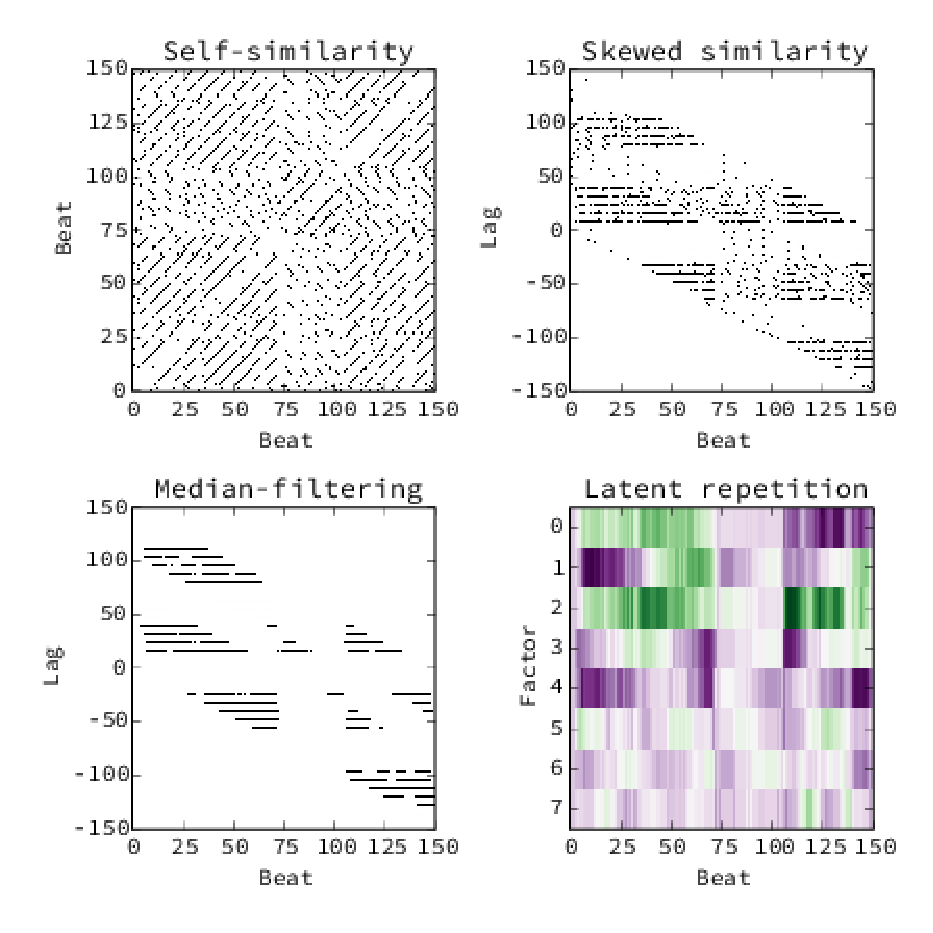
\includegraphics[width=\columnwidth]{figs/rep}
\vspace{-2\baselineskip}
\caption{Repetition features derived from \emph{Tupac Shakur --- Trapped}. 
Top-left: a binary self-similarity ($k$-nearest-neighbor) matrix over beats.
Top-right: the time-lag transformation of the self-similarity matrix.
Bottom-left: the result of the horizontal median filter.
Bottom-right: 8-dimensional latent factor representation (best viewed in color).}
\label{fig:rep}
\end{figure}

\subsection{Constrained agglomerative clustering}
\label{sec:clustering}
Given a feature matrix $X \in \R^{D\times t}$, we produce a hierarchical clustering of the columns of $X$ by using the
linkage-constrained variant of Ward's agglomerative clustering algorithm~\cite{ward1963hierarchical} as implemented in
\texttt{scikit-learn}~\cite{pedregosa2011scikit}.  For each column $X_{\cdot,i}$, linkage constraints are generated
for $(i-1, i)$ and $(i, i+1)$, so the linkage graph forms a chain.  Starting from $t$ clusters (one for each column of $X$), 
the two closest linked clusters are iteratively merged until only one remains.
The hierarchy is computed in $\Oh(t)$ merge operations, and due to the constraints, 
there are $\Oh(t)$ feasible merges at each step. 
Each merge operation takes time $\Oh(D + \log t)$ (to compute centroids and manage a priority queue), so the algorithm runs in $\Oh(tD + t\log t)$ time.
For $D \in \Omega(\log t)$, the cost of clustering is dominated by the $\Omega(tD)$ cost of computing $X$.

\subsection{Choosing the number of segments}
The hierarchical clustering produces segmentations for all numbers of segments $1 \leq k \leq t$.  While a multi-scale view can 
be useful in some scenarios --- such as interactive data exploration --- standard evaluations rely on flat segmentations. 
To select $k$, we compute the clustering cost of each pruning within a plausible bounded range 
$k_{\min} \leq k \leq k_{\max}$.  The bounds are determined by assuming average minimum and maximum segment duration 
of 10s and 45s.  AIC correction~\cite{akaike1973information} is then applied to each candidate pruning (assuming a spherical 
Gaussian model for each segment), and $k$ is chosen to minimize the AIC-corrected cost.

\subsection{Multiple features}
Structural repetition features are most commonly used to detect repeated chord sequences, but the idea is general enough to
support any kind of feature descriptor.  We aggregate several types of feature descriptors for each beat:
\begin{description}\addtolength{\itemsep}{-0.5\baselineskip}%
\item[MFCC]   Beat-synchronous (mean) Mel-frequency cepstral coefficients and their latent repetitions;
\item[Chroma] Beat-synchronous (median) chroma and their latent repetitions; and
\item[Time]   Time-stamp (in seconds) of each beat, normalized time-stamps (as a fraction of track duration), 
beat indices $(1, 2, \ldots, t)$, and normalized beat indices\\ $(1/t, 2/t, \ldots, 1)$.
\end{description}
The MFCC features capture local timbre, and repeated timbre sequences. 
Similarly, chroma features capture local pitch similarity and sequential repetitions.
The time features act as an implicit quadratic regularization on segment durations, and promote balanced segmentations.

All features can be stacked together into a single feature matrix $X \in \R^{D\times t}$, and clustered via the method described
above. However, the relative magnitude and importance of each feature is not calibrated to produce optimal clusterings. 

\section{Ordinal linear discriminant analysis}
\begin{table*}
\centering
\caption{Segmentation performance. Best scores are indicated in bold; significance is assessed with a Bonferroni-corrected Wilcoxon
signed-rank test at $\alpha=0.05$.\label{tab:results}}
\footnotesize
\begin{tabular}{lrrrrrrrrrrrr}
% \bottomrule%
\multicolumn{13}{c}{Beatles-ISO}\\
\toprule%
Algorithm   &   $P_{0.5s}$ & $R_{0.5s}$ & $F_{0.5s}$ & $P_{3s}$     & $R_{3s}$  & $F_{3s}$   & $S_O$ & $S_U$ & $S_F$ & $P_C$& $R_C$& $F_C$\\
\hline
Unweighted  & 
0.274 & 0.218 & 0.237 & 0.606 & 0.469 & 0.518 & \textbf{0.842} & 0.755 & 0.791 & \textbf{0.780} & 0.613 & 0.668\\
FDA         &  
0.275 & 0.208 & 0.229 & 0.582 & 0.430 & 0.483 & \textbf{0.839} & 0.778 & 0.802 & \textbf{0.774} & 0.653 & 0.691\\
OLDA        & 
\textbf{0.299} & \textbf{0.296} & \textbf{0.289} & 0.601 & 0.577 & 0.573 & 0.828 & 0.808 & 0.813 & 0.744 & 0.686 & 0.694\\
\hline
SMGA~\hfill\cite{serra2012unsupervised} &  
0.147 & 0.172 & 0.156 & \textbf{0.627} & \textbf{0.728} & \textbf{0.661} & 0.811 & \textbf{0.858} & \textbf{0.829} & 0.702 &
\textbf{0.798} & \textbf{0.729}\\
\toprule%
\multicolumn{13}{c}{SALAMI-free}\\
\toprule%
Unweighted  & 
0.236 & 0.184 & 0.200 & 0.495 & 0.390 & 0.422 & 0.812 & 0.795 & 0.794 & 0.666 & 0.652 & 0.626\\
FDA     & 
\textbf{0.296} & 0.166 & 0.205 & \textbf{0.564} & 0.330 & 0.400 & 0.849 & 0.729 & 0.771 & 0.751 & 0.566 & 0.603\\
OLDA    & 
0.265 & \textbf{0.234} & \textbf{0.241} & 0.510 & 0.457 & 0.467 & 0.804 & 0.829 & \textbf{0.808} & 0.640 & 0.707 & \textbf{0.640}\\
\hline
SMGA~\hfill\cite{serra2012unsupervised} &
0.115 & 0.178 & 0.134 & 0.434 & \textbf{0.666} & \textbf{0.508} & 0.714 & \textbf{0.895} & 0.786 & 0.448 & \textbf{0.822} & 0.550\\
C-NMF~\hfill\cite{nieto2013convex}  &
0.105 & 0.133 & 0.110 & 0.450 & 0.543 & 0.463 & 0.767 & 0.797 & 0.767 & 0.576 & 0.639 & 0.550\\
SI-PLCA~\hfill\cite{weiss2011unsupervised}  &
0.210 & 0.102 & 0.128 & 0.451 & 0.228 & 0.286 & \textbf{0.873} & 0.538 & 0.643 & \textbf{0.814} & 0.362 & 0.459\\
\bottomrule%
\end{tabular}
\end{table*}


\label{sec:olda}
To improve the feature representation for clustering, we propose a simple adaptation of Fisher's linear discriminant
analysis (FDA)~\cite{fisher1936use}.  In its multi-class form, FDA takes as input a labeled collection of data $x_i \in \R^D$
and class labels $y_i \in \{1,2,\ldots, C\}$, and produces a linear transformation $W \in \R^{D\times D}$ that simultaneously 
maximizes the distance between class centroids, and minimizes the variance of each class 
individually~\cite{fukunaga1990introduction}. This is accomplished by solving the following optimization:
\begin{equation}
W \defeq \argmax_W \trace\left( {(W\trans A_\text{W} W)}^{-1} W\trans A_\text{B} W \right) \label{eq:fda},
\end{equation}
where $A_\text{W}$ and $A_\text{B}$ are the \emph{within-} and \emph{between}-class scatter matrices:
\begin{align*}
A_\text{W} & \defeq \sum_c \sum_{i : y_i = c} (x_i - \mu_c)(x_i - \mu_c)\trans\\
A_\text{B} & \defeq \sum_c n_c (\mu_c - \mu)(\mu_c - \mu)\trans,
\end{align*}
$\mu$ denotes the mean across all classes, $\mu_c$ is the mean of class $c$, and $n_c$ denotes the number of examples in class $c$.
\Cref{eq:fda} can be efficiently solved as a generalized eigenvalue problem over the two scatter matrices $(A_\text{B},
A_\text{W})$~\cite{de2005eigenproblems}.

Class labels can be synthesized from segments on an annotated training song, so that the columns of $X$ belonging to the first 
segment are assigned to class 1, the second segment to class 2, and so on.
However, interpreting each segment as a distinct class could result in a repeated verse being treated as two distinct classes which 
cannot be separated. 
A more serious problem with this formulation is that it is unclear how to generalize across multiple songs, as it would result in
FDA attempting to separate segments from different songs, which is somewhat meaningless for the single-song segmentation task.

Now, note that due to linkage constraints, the agglomerative clustering algorithm (\cref{sec:clustering}) only considers merge 
operations over adjacent segments $(c, c+1)$. This motivates a relaxed FDA problem which only attempts to separate adjacent
segments.  This is accomplished by replacing the between-class scatter matrix $A_B$ with the resulting \emph{ordinal scatter matrix}:
\begin{align*}
A_\text{O} &\defeq \sum_{c < C} n_c (\mu_c - \mu_{c+}) (\mu_c - \mu_{c+})\trans\\
\mu_{c+} &\defeq \frac{n_c \mu_c + n_{c+1} \mu_{c+1} }{n_c + n_{c+1}}.
\end{align*}

Because $A_\text{W}$ may be rank-degenerate, we include a smoothing parameter
$\lambda > 0$.\footnote{The same regularization strategy is applied to FDA in \Cref{sec:eval}.} 
The OLDA optimization takes the form:
\begin{equation}
W \defeq \argmax_W \trace\left( {(W\trans (A_\text{W} + \lambda I) W)}^{-1} W\trans A_\text{O} W \right) \label{eq:olda},
\end{equation}
which again can be solved efficiently as a generalized eigenvalue problem over the matrix pair 
$(A_\text{O}, A_\text{W} + \lambda I)$.

Because interactions are only measured between neighboring segments, it is 
straightforward to include data from multiple songs by summing their individual contributions to $A_\text{O}$ and $A_\text{W}$.
After learning $W$, the feature matrix $X$ for a previously unseen song is transformed via $X \mapsto W\trans X$, and then 
clustered as described in \Cref{sec:clustering}.

\section{Evaluation}
\label{sec:eval}
All proposed methods are implemented in Python with the \texttt{librosa} package.\footnote{Code is
available at \url{https://github.com/bmcfee/olda}.}  
All signals were downsampled to 22KHz mono, and analyzed with a 93ms window and 3ms hop.  MFCCs are generated from 128 Mel bands
with an 8KHz cutoff. We take 32 MFCCs and 12 chroma bins; repetition features are calculated with $2\sqrt{t}$ nearest neighbors,
median-filtered with a window width of 7, and projected to 32 dimensions each.  Including the four time-stamp features, the combined
representation has dimension $D=112$. Beat tracking was done with the \emph{med-full} method described in~\cite{mcfee2014beat}.

\subsection{Data and metrics}
To evaluate the proposed methods, we evaluate predicted segmentations on two publicly available datasets:
\begin{description}\addtolength{\itemsep}{-0.25\baselineskip}%
\item[Beatles-ISO] 179 songs by the Beatles~\cite{harte2010towards,isophonicsbeatles}, and
\item[SALAMI-free] 253 songs from the SALAMI dataset~\cite{smith2011design} which are freely available on the 
Internet Archive~\cite{nieto2013convex}.
\end{description}
Both datasets provide labels for each annotated segment (\eg, \emph{verse} or \emph{intro}), but we ignore these
labels in this set of experiments. Compared to the Beatles corpus, SALAMI consists of tracks by multiple artists, 
and has much more diversity of genre, style, and instrumentation.

On both datasets, we compare to SMGA~\cite{serra2012unsupervised}, which achieved the
highest performance in the 2012 MIREX structural segmentation evaluation~\cite{Downie2008}.
On SALAMI-Free, we include comparisons to C-NMF~\cite{nieto2013convex} and SI-LPCA~\cite{weiss2011unsupervised}.

For both datasets, we evaluate the unweighted feature representation (\emph{Unweighted}), FDA optimization (using the
one-class-per-segment approach described in \Cref{sec:olda}), and OLDA.\@
To ensure fairness of evaluation, the FDA and OLDA models used on the Beatles-ISO were trained using only
SALAMI-free data, and vice versa.  FDA and OLDA were trained with $\lambda \in \{10^0, 10^1, \dots, 10^7\}$, 
and choosing the $\lambda$ which maximized $S_F$ score (see below) on the training set.

We report the following standard segmentation metrics:
\footnote{For a detailed description of segmentation metrics, see~\cite{mirexstructure}.}
\begin{description}\addtolength{\itemsep}{-0.25\baselineskip}%
\item[Boundary retrieval] Precision, recall, and F-measure at both 0.5s and 3s resolution,
\item[Normalized conditional entropy] (NCE) Over- and under-segmentation scores $S_O$ and $S_U$, and their harmonic
mean $S_F$, and
\item[Frame clustering] Precision ($P_C$), recall ($R_C$), and F-measure ($F_C$) of detecting whether any two frames 
belong to the same segment.
\end{description}
Note that boundary retrieval and frame clustering metrics are highly sensitive to changes in the number of
predicted segments, upon which multiple human annotators often disagree for the same track. 
The NCE metrics are designed to be fairly robust to changes in segmentation granularity.
Following MIREX practice, frames are sampled at a frequency of 10Hz for the NCE and frame clustering metrics. 


\subsection{Results}
\label{sec:results}

\Cref{tab:results} lists the results for the Beatles-ISO and SALAMI-free.
SMGA performs best on the majority of metrics for Beatles-ISO (\cref{tab:results}, top),\footnote{SMGA parameters were selected to 
perform well on the Beatles data~\cite{serra2012unsupervised}.}
The scores on the NCE metrics ($S_O, S_U, S_F$) are qualitatively comparable between SMGA and OLDA ($S_F$ of 0.829 and 0.813, respectively),
suggesting that SMGA and the proposed methods are producing segmentations of comparable quality, but different levels of granularity.
The unweighted, FDA, and OLDA models all achieve higher accuracy for boundary detection at 0.5s resolution.

Results on the SALAMI-free data (\cref{tab:results}, bottom) are mixed, though the FDA and OLDA methods both show marked
improvement over the unweighted method.  Overall, the OLDA model tends to achieve a better balance between precision and recall
than FDA, and achieves maximal F-scores on all but 3s boundary detection. 

\section{Conclusion}
\label{sec:conclusion}


\bibliographystyle{IEEEbib}
\bibliography{refs}

\end{document}
